\documentclass[../Presentation.tex]{subfiles}
\usepackage[utf8]{inputenc}
\title{Estructura de Datos}
\subtitle{Estructura de Datos en C}
\author{José Everardo Torres O.}
\usetheme{lucid}

\begin{document}
\frame{
\titlepage
}
\frame {
\frametitle{Listas Enlazadas}
\section{Listas Enlazadas}
Vamos a suponer que tenemos los siguientes 5 elementos:
\begin{center}
1,2,4,5
\end{center}
y queremos introducir el 3 entre el valor 2 y 4. En el arreglo, no podemos hacer esto facilmente. Para eso necesitamos una lista enlazada que nos permita añadir elementos.
\begin{figure}
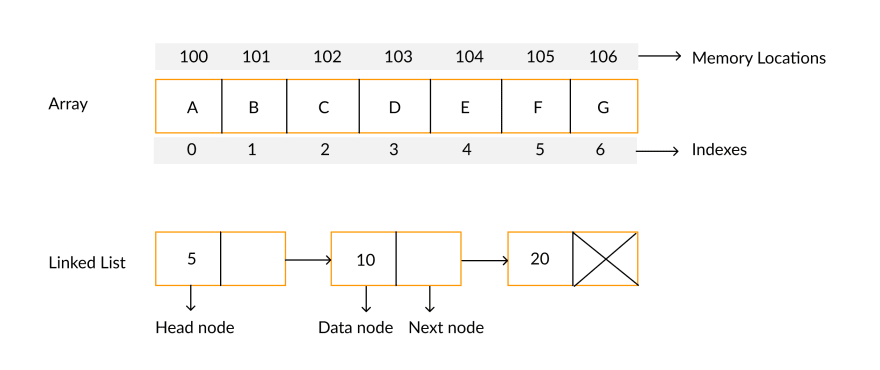
\includegraphics[scale=0.2]{ArrayVsLinkedList}
\caption{\label{fig:ArrayvsList} Un Array vs Una Linked List}
\end{figure}

\note{El arreglo es una estructura de datos lineal, que no se puede modificar una vex que se haya creado. Para añadir el 3 tendriamos que crear otro arreglo con un espacio adicional donde podamos añadir el 3. Esta operación de copiar los elementos es infeficiente. Para remover esa ineficiencia usamos listas enlazadas.}}
\frame{
\frametitle{Lista Enlazada}
\subsection{Lista Enlazada}
Una lista enlazada es una lista de elementos, llamados nodos. Lo nodos tienen dos partes, La parte del valor (Tipo de dato) que es usada para almacenar los datos, y la parte del enlace (Apuntador al siguiente elemento) que es usado para almacenar la dirección de memoria del siguiente elemento de la lista.
\begin{figure}
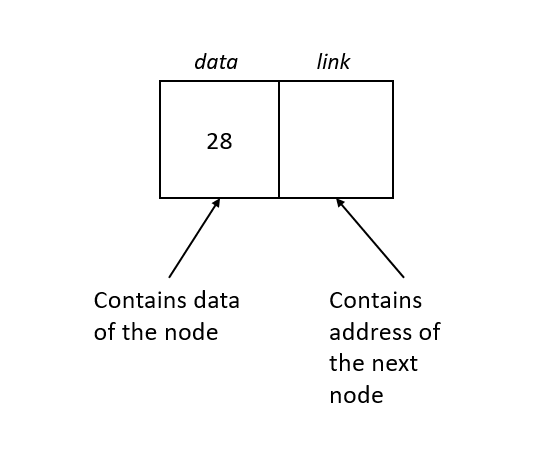
\includegraphics[scale=.2]{Node}
\caption{\label{fig:NodeList} Un Nodo de Lista}
\end{figure}
\note{La lista enlazada es el elemento más basicos de las listas.}
}
\frame{
\frametitle{Tipos de Listas}
\subsection{Tipos de Listas}
Existen diferentes tipos de listas. La principal entre ellos es como los nodos se refieren a otros nodos.
\begin{itemize}
\item Lista Enlazada Individualmente (Singly Linked List)
\item Lista Enlazada Doblemente (Double Linked List)
\item Lista Enlazada Circularmente (Circular Linked List)
\end{itemize}
\note{A Continuación se describiran los tipos de listas, este es un pequeño menu con los tipos de listas}
}

\end{document}